% This file was created with tikzplotlib v0.10.1.
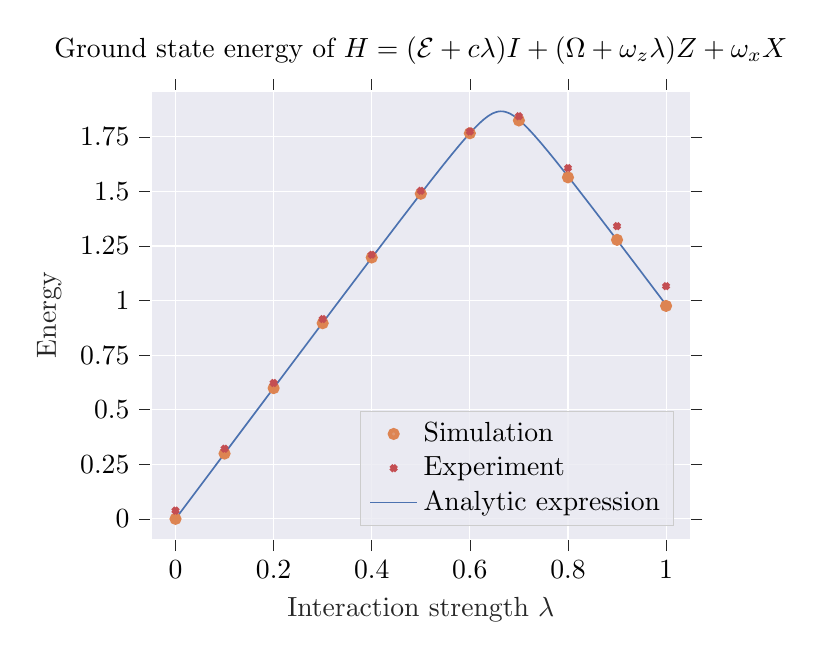
\begin{tikzpicture}

\definecolor{darkslategray38}{RGB}{38,38,38}
\definecolor{indianred1967882}{RGB}{196,78,82}
\definecolor{lavender234234242}{RGB}{234,234,242}
\definecolor{lightgray204}{RGB}{204,204,204}
\definecolor{peru22113282}{RGB}{221,132,82}
\definecolor{steelblue76114176}{RGB}{76,114,176}

\begin{axis}[
axis background/.style={fill=lavender234234242},
axis line style={white},
legend cell align={left},
legend style={
  fill opacity=0.8,
  draw opacity=1,
  text opacity=1,
  at={(0.97,0.03)},
  anchor=south east,
  draw=lightgray204,
  fill=lavender234234242
},
mark options={mark size=1.4pt, line width=1.5pt},
minor xtick={},
minor ytick={},
tick align=outside,
title style={align=center},
title={Ground state energy of \(\displaystyle H = (\mathcal{E}+ c\lambda)I + (\Omega + \omega_z\lambda) Z + \omega_x X\)},
x grid style={white},
xlabel=\textcolor{darkslategray38}{Interaction strength \(\displaystyle \lambda\)},
xmajorgrids,
xmajorticks=false,
xmajorticks=true,
xmin=-0.05, xmax=1.05,
xtick style={color=darkslategray38},
xtick={-0.2,0,0.2,0.4,0.6,0.8,1,1.2},
y grid style={white},
ylabel=\textcolor{darkslategray38}{Energy},
ymajorgrids,
ymajorticks=false,
ymajorticks=true,
ymin=-0.093347962718084, ymax=1.96030721707976,
ytick style={color=darkslategray38},
ytick={-0.25,0,0.25,0.5,0.75,1,1.25,1.5,1.75,2}
]
\addplot [draw=peru22113282, fill=peru22113282, mark=*, only marks]
table{%
x  y
0 0
0.1 0.299150390625
0.2 0.5990234375
0.3 0.89642578125
0.4 1.1974609375
0.5 1.48935546875
0.6 1.76640625
0.7 1.8251171875
0.8 1.5644921875
0.9 1.278193359375
1 0.9755859375
};
\addlegendentry{Simulation}
\addplot [draw=indianred1967882, fill=indianred1967882, mark=x, only marks]
table{%
x  y
0 0.0380859375
0.1 0.32130859375
0.2 0.62240234375
0.3 0.915244140625
0.4 1.20984375
0.5 1.50283203125
0.6 1.7744921875
0.7 1.8446484375
0.8 1.6072265625
0.9 1.34078125
1 1.066015625
};
\addlegendentry{Experiment}
\addplot [semithick, steelblue76114176]
table {%
0 0
0.200999975204468 0.602421760559082
0.322000026702881 0.963996410369873
0.401000022888184 1.19897496700287
0.455000042915344 1.35851263999939
0.49399995803833 1.4726619720459
0.523000001907349 1.5564888715744
0.546000003814697 1.62188804149628
0.564000010490417 1.67199409008026
0.578000068664551 1.7099666595459
0.589999914169312 1.74149656295776
0.600000023841858 1.76676189899445
0.608000040054321 1.7860780954361
0.615000009536743 1.802126288414
0.621000051498413 1.81508207321167
0.626999974250793 1.82712388038635
0.631999969482422 1.83631443977356
0.635999917984009 1.8430163860321
0.639999985694885 1.84905624389648
0.644000053405762 1.85435163974762
0.647000074386597 1.85778415203094
0.649999976158142 1.86071610450745
0.652999997138977 1.86311554908752
0.656000018119812 1.86495387554169
0.658999919891357 1.86620819568634
0.66100001335144 1.86671149730682
0.662999987602234 1.8669445514679
0.664999961853027 1.86690604686737
0.66700005531311 1.86659622192383
0.669000029563904 1.8660169839859
0.671000003814697 1.86517179012299
0.674000024795532 1.86341655254364
0.677000045776367 1.86109662055969
0.680000066757202 1.85823965072632
0.683000087738037 1.85487747192383
0.685999989509583 1.85104417800903
0.690000057220459 1.84526145458221
0.694000005722046 1.83878755569458
0.699000000953674 1.82984411716461
0.703999996185303 1.82008707523346
0.710000038146973 1.80747985839844
0.717000007629395 1.79175841808319
0.725000023841858 1.77273368835449
0.733999967575073 1.75029170513153
0.745000004768372 1.72174477577209
0.758000016212463 1.68685698509216
0.773000001907349 1.64551138877869
0.79200005531311 1.59199690818787
0.815999984741211 1.52320003509521
0.845999956130981 1.43602073192596
0.884999990463257 1.32150602340698
0.937999963760376 1.16466188430786
0.999000072479248 0.983176946640015
};
\addlegendentry{Analytic expression}
\end{axis}

\end{tikzpicture}
